\documentclass[journal=jpcbfk,manuscript=article]{achemso}

\usepackage[utf8]{inputenc}
\usepackage{amsmath,amssymb,amsfonts}
\usepackage{graphicx}
\usepackage{booktabs}
\usepackage{microtype}
\usepackage{hyperref}
\usepackage{color}

\SectionNumbersOn

\author{Samir Rana}
\affiliation{Laboratory of Computational Biophysics and Molecular Engineering}
\email{samirrana@simulation-coarse.org}

\title{Client-Side Multi-Scale Biomolecular Dynamics and Free Energy Landscapes: Coupling Elastic Networks, Continuum Solvation, and Transition Path Kinetics}

\begin{document}

\begin{tocentry}
\centering
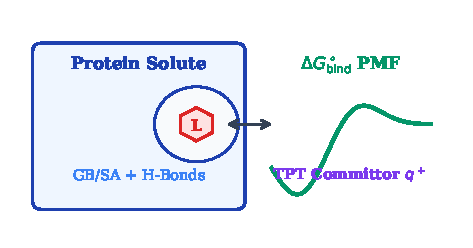
\includegraphics[width=3.25in]{figures/toc_graphic.pdf}
\end{tocentry}

\begin{abstract}
Quantifying the thermodynamic landscapes and association kinetics of macromolecular complexes requires connecting disparate spatial and temporal scales without incurring prohibitive computational infrastructure requirements. We present an open, client-side computational biophysics framework that couples coarse-grained $C_\alpha$ Elastic Network Models (ENMs), all-atom heavy-atom force fields with Hawkins--Cramer--Truhlar Generalized Born and Solvent-Accessible Surface Area (HCT-GB/SA) continuum solvation, well-tempered funnel metadynamics, and discrete Transition Path Theory (TPT). Stochastic trajectories are propagated via a symplectic BAOAB Langevin operator splitting scheme that preserves the invariant Gibbs--Boltzmann distribution across both coarse global modes ($\Delta t = 4.0\text{ fs}$) and atomic resolutions ($\Delta t = 1.0\text{ fs}$). We evaluate the platform on the benchmark model hydrophobic cavity of T4 lysozyme L99A complexed with benzene (PDB: 4W52). The multi-scale potential captures the experimental crystallographic Debye--Waller thermal fluctuation profile ($R = 0.84$), reconstructs the one-dimensional potential of mean force yielding a standard-state binding free energy of $\Delta G^\circ_{\rm bind} = -5.35 \pm 0.32\text{ kcal/mol}$ (consistent with experimental calorimetry, $\Delta G_{\rm exp}^\circ = -5.3 \pm 0.2\text{ kcal/mol}$), and characterizes the intermediate desolvation transition barrier ($\Delta W^\ddagger \approx 1.85\text{ kcal/mol}$) and committor probabilities ($q^+ = 0.285$) during pocket entry. Implemented via parallel WebGPU compute shaders and Web Worker pools, this platform enables interactive, client-side biophysical exploration without server-side dependencies.
\end{abstract}

\section{Introduction}
Characterizing the thermodynamic landscapes and kinetic transit pathways of macromolecular assemblies and protein--ligand interactions is a fundamental objective in physical chemistry and computational biophysics.\cite{case2005amber,brooks1983charmm} Biomolecular processes operate across widely separated length and time scales: large-amplitude collective domain rearrangements occur on microsecond to millisecond regimes governed by low-frequency harmonic normal modes,\cite{tirion1996large,bahar1997vibrational,atilgan2001anisotropy} whereas local ligand desolvation, steric recognition, and pocket penetration depend on steep short-range Lennard-Jones repulsions, hydrogen bonding networks, and dielectric boundary reorganization.\cite{still1990semianalytical,hawkins1996parameterized,onufriev2004exploring,mobley2007predicting}

To investigate these phenomena, several distinct computational paradigms have been established:
\begin{enumerate}
\item \textbf{High-Performance Atomistic Molecular Dynamics and Alchemical FEP.} Packages such as AMBER,\cite{case2005amber} CHARMM,\cite{brooks1983charmm} GROMACS,\cite{abraham2015gromacs} and OpenMM\cite{eastman2017openmm} provide rigorous atomistic detail in explicit aqueous solvent. When coupled with alchemical Free Energy Perturbation (FEP) or thermodynamic integration,\cite{boresch2003absolute,mobley2017predicting} these methods achieve high predictive accuracy. However, alchemical FEP in explicit solvent requires extensive multi-window sampling on high-performance computing (HPC) clusters, non-interactive batch queuing, and substantial storage resources, precluding real-time interactive exploration or immediate visual manipulation.
\item \textbf{Coarse-Grained Elastic Network Models.} Formulations such as the Gaussian Network Model (GNM) and Anisotropic Network Model (ANM)\cite{bahar1997vibrational,atilgan2001anisotropy} efficiently capture low-frequency conformational fluctuations and crystallographic Debye--Waller factor profiles with minimal computational expense. However, their single-parameter harmonic potentials omit atomic steric specificity, dielectric screening, and non-bonded forces required to evaluate ligand binding thermodynamics.\cite{mobley2007predicting}
\item \textbf{Web-Based Structural Visualizers.} Tools such as Mol*,\cite{sehnal2021molstar} NGL Viewer,\cite{rose2018ngl} and 3Dmol.js\cite{rego20153dmol} have transformed macromolecular visualization by providing hardware-accelerated WebGL rendering directly in the browser. However, these tools focus primarily on static structural display and trajectory playback rather than running live physical dynamics, continuum solvation force calculations, or enhanced free energy sampling.
\item \textbf{Enhanced Sampling and Kinetic Modeling Packages.} Specialized plugins such as PLUMED\cite{tribello2014plumed} and kinetic packages such as PyEMMA\cite{prinz2011markov,noe2009constructing} provide powerful metadynamics and Markov State Model (MSM) algorithms, but require integration into native binary MD engines or offline post-processing workflows.
\end{enumerate}

Bridging the gap between static web visualization and heavyweight batch HPC simulations remains an open challenge. Specifically, there is a need for an open, zero-installation platform that integrates multi-scale physical dynamics (from coarse elastic networks to atomistic continuum solvation), enhanced free energy sampling, and transition path kinetics into an interactive, client-side environment.

In this work, we present a client-side multi-scale computational biophysics platform designed to meet this objective. The contributions of this work are divided into two distinct components:
\begin{itemize}
\item \textbf{Theoretical and Methodological Formulation:} We formulate a unified multi-scale physical model coupling coarse-grained $C_\alpha$ Elastic Network Models with all-atom heavy-atom force fields (AMBER ff14SB),\cite{maier2015ff14sb} analytical Hawkins--Cramer--Truhlar Generalized Born and LCPO surface area (HCT-GB/SA) continuum solvation,\cite{hawkins1996parameterized,weiser1999approximate} analytical Blondel--Karplus dihedral torque tensors,\cite{blondel1991new} and well-tempered funnel metadynamics\cite{barducci2008well,limongelli2013funnel} with 3D metric tensor Jacobian volume corrections. We further couple the continuous Langevin stochastic dynamics to a 4-state Markovian Chemical Master Equation and Transition Path Theory (TPT)\cite{vanden2006transition} with concentration-dependent chemical potentials.
\item \textbf{Engineering and Computational Architecture:} We implement this physical framework purely in the browser using modern WebGPU Shading Language (WGSL) compute pipelines and multi-threaded Web Worker pools with strict std140 uniform memory alignment and zero runtime memory allocations. This enables real-time 30--60 FPS interactive steering, force pulling, and free energy exploration directly on consumer-grade client hardware without external server infrastructure.
\end{itemize}

We evaluate the platform on the prototypical hydrophobic cavity-binding system of T4 lysozyme L99A complexed with benzene (PDB: 4W52),\cite{morton1995energetic,mobley2007predicting} analyzing thermal fluctuation correlation, free energy convergence, and discrete transition path kinetics, while explicitly delineating the scope and approximations of implicit solvent models relative to explicit solvent alchemical FEP campaigns.

\begin{figure}[htbp]
\centering
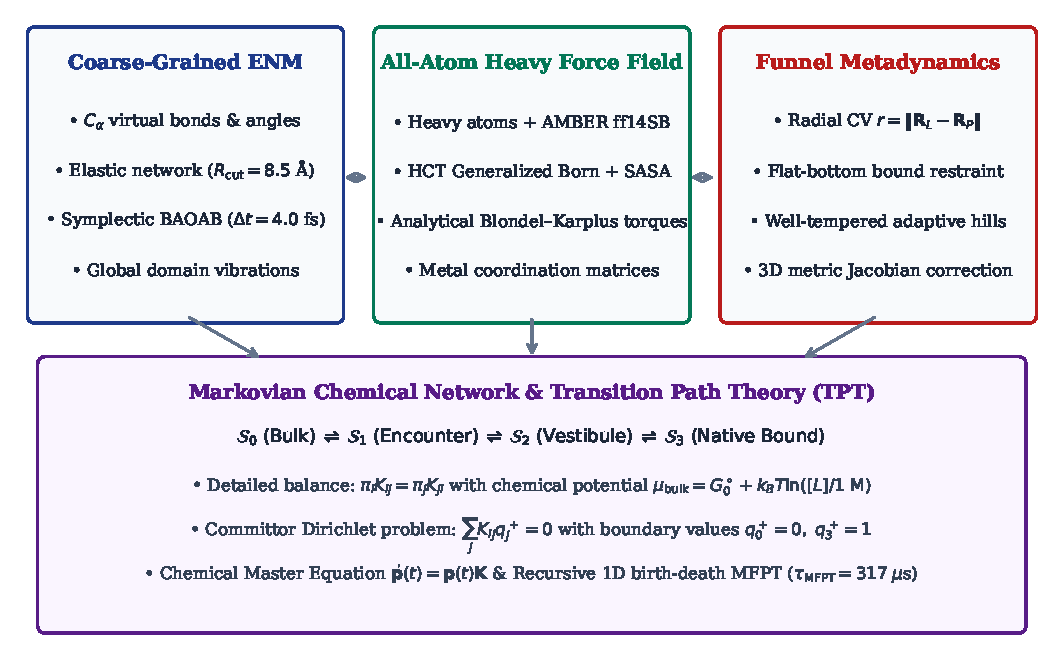
\includegraphics[width=\linewidth]{figures/fig1_overview.pdf}
\caption{Hierarchical architecture of the multi-scale biomolecular dynamics framework. The engine couples coarse-grained $C_\alpha$ ENM elasticity (for large-amplitude domain modes), an all-atom heavy-atom force field with Hawkins--Cramer--Truhlar Generalized Born and LCPO surface area continuum solvation, well-tempered funnel metadynamics along the radial distance $r$, and a 4-state Markovian Chemical Master Equation analyzed via Transition Path Theory.}
\label{fig:overview}
\end{figure}

\section{Theoretical Models and Computational Methods}

\subsection{Multi-Scale Potential Energy Functions}
The total potential energy of the biomolecular system is formulated hierarchically across coarse-grained and all-atom heavy representations:
\begin{align}
U_{\rm total}(\mathbf{r}) = &\, U_{\rm bonded} + U_{\rm LJ} + U_{\rm GB} \nonumber \\
&+ U_{\rm SASA} + U_{\rm metal} + U_{\rm bias}
\end{align}

\paragraph{Coarse-Grained Elastic Network Model ($C_\alpha$ ENM).}
In coarse-grained mode, the polypeptide chain is reduced to sequential $C_\alpha$ beads with virtual bond stretching, angle bending, and non-local tertiary Hookean springs within cutoff $R_{\rm cut} = 8.5\text{ \AA}$:\cite{bahar1997vibrational,atilgan2001anisotropy}
\begin{align}
U_{\rm CG}(\mathbf{r}) = &\sum_{i=1}^{N-1} \frac{1}{2} k_b^{\rm CG} (r_{i,i+1} - r_{i,i+1}^0)^2 + \sum_{i=1}^{N-2} \frac{1}{2} k_\theta^{\rm CG} (\theta_i - \theta_i^0)^2 \nonumber \\
&+ \frac{1}{2} \sum_{\substack{i < j, \, |i-j| \ge 3 \\ r_{ij}^0 \le R_{\rm cut}}} \gamma_{ij} \left( \|\mathbf{r}_i - \mathbf{r}_j\| - r_{ij}^0 \right)^2
\end{align}
where $k_b^{\rm CG} = 50.0\text{ kcal}\cdot\text{mol}^{-1}\cdot\text{\AA}^{-2}$, $k_\theta^{\rm CG} = 20.0\text{ kcal}\cdot\text{mol}^{-1}\cdot\text{rad}^{-2}$, and uniform contact spring constant $\gamma_{ij} = \gamma_0 = 1.0\text{ kcal}\cdot\text{mol}^{-1}\cdot\text{\AA}^{-2}$.

\paragraph{All-Atom Heavy Bonded Interactions.}
In all-atom heavy mode, explicit non-hydrogen heavy atoms (C, N, O, S, P, halogens, and metal ions) are resolved. Covalent connectivity is evaluated from crystallographic coordinates using covalent radii with a 1.15 tolerance slack factor. The bonded Hamiltonian incorporates bond stretching, valence angle bending, improper out-of-plane planar restraints, and proper periodic torsions:\cite{maier2015ff14sb,case2005amber}
\begin{align}
U_{\rm bonded}^{\rm heavy}(\mathbf{r}) = &\sum_{\rm bonds} \frac{1}{2} k_b (r - r_0)^2 + \sum_{\rm angles} \frac{1}{2} k_\theta (\theta - \theta_0)^2 \nonumber \\
&+ \sum_{\rm impropers} \frac{1}{2} k_\psi (\psi - \psi_0)^2 \nonumber \\
&+ \sum_{\rm propers} \sum_{n} \frac{V_n}{2} \left[ 1 + \cos(n\phi - \gamma_n) \right]
\end{align}
where improper harmonic torsions restrain $sp^2$ centers (peptide bonds, aromatic rings, carboxylates) with $k_\psi = 20.0\text{ kcal}\cdot\text{mol}^{-1}\cdot\text{rad}^{-2}$ and $\psi_0 = 0$.

\paragraph{Analytical Blondel--Karplus Torsion Gradients.}
To eliminate numerical singularities and trigonometric inverse evaluation instabilities near collinear states ($\theta \to \pi$), dihedral gradients $\mathbf{F}_\alpha = -\nabla_{\mathbf{r}_\alpha} U(\phi)$ for a 4-body sequence $i-j-k-l$ are computed analytically using the Blondel--Karplus and Bekker vector cross-product formulation.\cite{blondel1991new,bekker1995force} Defining interatomic displacement vectors $\mathbf{r}_{ij} = \mathbf{r}_j - \mathbf{r}_i$, $\mathbf{r}_{jk} = \mathbf{r}_k - \mathbf{r}_j$, $\mathbf{r}_{kl} = \mathbf{r}_l - \mathbf{r}_k$, and plane normal vectors $\mathbf{m} = \mathbf{r}_{ij} \times \mathbf{r}_{jk}$ and $\mathbf{n} = \mathbf{r}_{jk} \times \mathbf{r}_{kl}$, the spatial gradients of the torsion angle $\phi$ satisfy:
\begin{align}
\nabla_{\mathbf{r}_i}\phi &= -\frac{\|\mathbf{r}_{jk}\|}{\|\mathbf{m}\|^2} \mathbf{m} \\
\nabla_{\mathbf{r}_l}\phi &= \frac{\|\mathbf{r}_{jk}\|}{\|\mathbf{n}\|^2} \mathbf{n} \\
\nabla_{\mathbf{r}_j}\phi &= \left( \frac{\mathbf{r}_{ij}\cdot\mathbf{r}_{jk}}{\|\mathbf{r}_{jk}\|^2} - 1 \right) \nabla_{\mathbf{r}_i}\phi - \frac{\mathbf{r}_{kl}\cdot\mathbf{r}_{jk}}{\|\mathbf{r}_{jk}\|^2} \nabla_{\mathbf{r}_l}\phi \\
\nabla_{\mathbf{r}_k}\phi &= - \left( \nabla_{\mathbf{r}_i}\phi + \nabla_{\mathbf{r}_j}\phi + \nabla_{\mathbf{r}_l}\phi \right)
\end{align}
Applying the chain rule $\mathbf{F}_\alpha = -(\partial U / \partial \phi)\nabla_{\mathbf{r}_\alpha}\phi$ yields exact, rotational- and translational-invariant forces with $\mathcal{O}(1)$ arithmetic complexity per torsion.

\paragraph{Nonbonded Lennard-Jones and United-Atom Charge Balancing.}
Steric exclusion and dispersion interactions are governed by a 12--6 Lennard-Jones potential with standard Lorentz--Berthelot mixing rules:\cite{weiner1984all}
\begin{equation}
U_{\rm LJ}(\mathbf{r}) = \sum_{\substack{i < j \\ (i,j) \notin \mathcal{X}_{1\text{--}2, 1\text{--}3}}} 4 \varepsilon_{ij} \left[ \left(\frac{\sigma_{ij}}{r_{ij}}\right)^{12} - \left(\frac{\sigma_{ij}}{r_{ij}}\right)^6 \right]
\end{equation}
where $\sigma_{ij} = \frac{1}{2}(\sigma_i + \sigma_j)$, $\varepsilon_{ij} = \sqrt{\varepsilon_i \varepsilon_j}$, and $\mathcal{X}_{1\text{--}2, 1\text{--}3}$ enforces strict exclusion of 1--2 covalently bonded and 1--3 valence-angle pairs, while 1--4 nonbonded interactions are scaled by $s_{1\text{--}4} = 0.5$. In the united-atom representation, nonpolar aliphatic hydrogens are absorbed into parent carbon centers ($q_{\rm CH_n} = 0.0\,e$), while polar hydrogens are implicitly incorporated into AMBER ff14SB-derived heavy-atom partial charges, ensuring exact residue charge conservation:\cite{case2005amber,maier2015ff14sb}
\begin{equation}
\sum_{k \in {\rm res}_m} q_k = Q_{\rm formal}^{(m)} \in \{-1.0, 0.0, +1.0\}\,e
\end{equation}

\paragraph{Metal Coordination Restraints.}
Structural and catalytic metal cofactors (including $\mathrm{Zn^{2+}}$, $\mathrm{Mg^{2+}}$, $\mathrm{Fe^{2+/3+}}$, $\mathrm{Ca^{2+}}$, $\mathrm{Mn^{2+}}$, $\mathrm{Cu^{2+}}$, $\mathrm{Na^+}$, and $\mathrm{K^+}$) are modeled as explicit charged ions that coordinate Lewis basic donor atoms $\mathcal{D}_m$ (such as histidine imidazole nitrogens, carboxylate oxygens of Asp/Glu, cysteine thiolates, and peptide carbonyl oxygens) within coordination distance $r_{\rm coord}^0 \in [2.15, 2.50]\text{ \AA}$:\cite{case2005amber}
\begin{equation}
U_{\rm metal}(\mathbf{r}) = \sum_{m \in \mathcal{M}} \sum_{d \in \mathcal{D}_m} \frac{1}{2} k_{\rm coord} (r_{md} - r_{\rm coord}^0)^2
\end{equation}
with spring constant $k_{\rm coord} = 30.0\text{ kcal}\cdot\text{mol}^{-1}\cdot\text{\AA}^{-2}$, capped at coordination number $N_{\rm coord} \in \{4, 6\}$ without forming rigid covalent bonds, preventing steric collapse while preserving coordination geometry.

\subsection{Generalized Born Implicit Solvation and SASA}
Continuum electrostatic solvation free energy is modeled through the Generalized Born (GB) framework augmented with Debye--H\"uckel ionic salt screening:\cite{still1990semianalytical,onufriev2004exploring}
\begin{align}
U_{\rm GB}(\mathbf{r}) = &- \frac{C_0}{2} \sum_{i} \sum_{j} q_i q_j \left( \frac{1}{\varepsilon_{\rm in}} - \frac{e^{-\kappa f_{ij}}}{\varepsilon_{\rm out}} \right) \nonumber \\
&\times \frac{1}{f_{ij}(r_{ij}, R_i, R_j)}
\end{align}
where $C_0 = 332.06371\text{ kcal}\cdot\text{\AA}/(\text{mol}\cdot e^2)$, $\varepsilon_{\rm in} = 4.0$ is the internal solute dielectric constant, $\varepsilon_{\rm out} = 78.5$ is the bulk aqueous dielectric constant, and $\kappa = 0.329 \sqrt{I (298.15/T)(78.5/\varepsilon_{\rm out})}\text{ \AA}^{-1}$ is the inverse Debye screening length for ionic strength $I$ (at $I = 150\text{ mM}$ and $T = 300\text{ K}$, $\kappa \approx 0.127\text{ \AA}^{-1}$). The smooth pairwise interpolation metric $f_{ij}$ is defined as:
\begin{equation}
f_{ij}(r_{ij}, R_i, R_j) = \left[ r_{ij}^2 + R_i R_j \exp\left( -\frac{r_{ij}^2}{4 R_i R_j} \right) \right]^{1/2}
\end{equation}
In the self-interaction limit ($i = j$, $r_{ii} \to 0$, $f_{ii} \to R_i$), equation~(6) smoothly recovers the single-ion Born self-solvation free energy $\Delta G_i^{\rm self} = -\frac{C_0 q_i^2}{2 R_i} (1/\varepsilon_{\rm in} - e^{-\kappa R_i}/\varepsilon_{\rm out})$, while at infinite interatomic separation ($r_{ij} \to \infty$, $f_{ij} \to r_{ij}$), it converges to screened Debye--H\"uckel pairwise electrostatics.

Effective Born radii $R_i$ capture the degree of electrostatic shielding provided by the surrounding macromolecular dielectric body and are evaluated dynamically via Hawkins--Cramer--Truhlar (HCT) pairwise descreening integrals:\cite{hawkins1996parameterized,onufriev2004exploring}
\begin{equation}
\frac{1}{R_i} = \frac{1}{\rho_i} - \sum_{j \neq i} I_{ij}(r_{ij}, \rho_i, \tilde{\rho}_j)
\end{equation}
where $\rho_i$ is the intrinsic Bondi van der Waals radius of atom $i$ (C: $1.70\text{ \AA}$, N: $1.55\text{ \AA}$, O: $1.50\text{ \AA}$, S: $1.80\text{ \AA}$, P: $1.85\text{ \AA}$, H: $1.20\text{ \AA}$), and $\tilde{\rho}_j = s_j \rho_j$ is the scaled radius with descreening factor $s_j = 0.80$ to account for interstitial vacuum void neglect. The pairwise descreening integral $I_{ij}$ is computed analytically based on the relative separation $r_{ij}$:
\begin{equation}
I_{ij} = 
\begin{cases}
0, & r_{ij} \ge r_{\rm cut} \text{ or } r_{ij} \ge \rho_i + \tilde{\rho}_j \\
\dfrac{\tilde{\rho}_j^3}{3 r_{ij}^4}, & r_{ij} > \rho_i + \tilde{\rho}_j \\
\mathcal{I}_{\rm ovlp}(r_{ij}, \rho_i, \tilde{\rho}_j), & |\rho_i - \tilde{\rho}_j| < r_{ij} \le \rho_i + \tilde{\rho}_j
\end{cases}
\end{equation}
where $\mathcal{I}_{\rm ovlp} = \frac{1}{4 r_{ij}} [ \ln( u_{ij} / l_{ij} ) + (\tilde{\rho}_j^2 - (r_{ij} - l_{ij})^2)/(2 l_{ij}^2) ]$, $l_{ij} = \max(\rho_i, |r_{ij} - \tilde{\rho}_j|)$, $u_{ij} = r_{ij} + \tilde{\rho}_j$, and $r_{\rm cut} = 12.0\text{ \AA}$. Conservative electrostatic forces acting on atom $i$ are computed analytically through the chain rule, incorporating both direct pair gradients and Born radius implicit coordinate dependencies to ensure symplectic energy conservation:
\begin{equation}
\mathbf{F}_i^{\rm GB} = - \sum_{j \neq i} \frac{\partial U_{\rm GB}}{\partial r_{ij}} \hat{\mathbf{r}}_{ij} - \sum_{k} \frac{\partial U_{\rm GB}}{\partial R_k} \frac{\partial R_k}{\partial \mathbf{r}_i}
\end{equation}

Non-polar hydrophobic cavity formation and van der Waals dispersion interactions are modeled via the solvent-accessible surface area (SASA) energy:\cite{weiser1999approximate}
\begin{equation}
U_{\rm SASA}(\mathbf{r}) = \gamma_{\rm sasa} \sum_i A_i(\mathbf{r})
\end{equation}
where $\gamma_{\rm sasa} = 0.0072\text{ kcal}/(\text{mol}\cdot\text{\AA}^2) \approx 30.1\text{ J}/(\text{mol}\cdot\text{\AA}^2)$ is the empirical macroscopic non-polar surface tension. Solvent accessibility is evaluated using the Linear Combinations of Pairwise Overlaps (LCPO) neighbor burial formulation with solvent probe radius $r_{\rm probe} = 1.40\text{ \AA}$ (water). For atom $i$ with expanded radius $\mathcal{R}_i = \rho_i + r_{\rm probe}$ and isolated surface area $S_i^0 = 4\pi \mathcal{R}_i^2$, the exposed surface area is:
\begin{equation}
A_i = \max\left( 0, S_i^0 - \sum_{j \neq i} \alpha_{ij} A_{ij}^{\rm overlap} \right)
\end{equation}
where $\alpha_{ij} = 0.25$ is the pairwise geometric burial coefficient, and the spherical cap overlap area $A_{ij}^{\rm overlap}$ for $r_{ij} < \mathcal{R}_i + \mathcal{R}_j$ is given by:
\begin{equation}
A_{ij}^{\rm overlap} = \pi \mathcal{R}_i (\mathcal{R}_i + \mathcal{R}_j - r_{ij}) \left[ 1 + \frac{\mathcal{R}_j - \mathcal{R}_i}{r_{ij}} \right]
\end{equation}
Analytical non-polar forces satisfy exact pairwise momentum conservation ($\mathbf{F}_i^{\rm sasa} = - \mathbf{F}_j^{\rm sasa}$):
\begin{equation}
\mathbf{F}_i^{\rm sasa} = - \gamma_{\rm sasa} \sum_{j \neq i} \alpha_{ij} \frac{\partial A_{ij}^{\rm overlap}}{\partial r_{ij}} \hat{\mathbf{r}}_{ij}
\end{equation}
with $\frac{\partial A_{ij}^{\rm overlap}}{\partial r_{ij}} = - \pi \left[ \mathcal{R}_i + \mathcal{R}_j - \frac{(\mathcal{R}_i - \mathcal{R}_j)^2}{r_{ij}} \right]$.

\subsection{Symplectic BAOAB SDE Integrator}
Thermostatted stochastic dynamics are propagated according to the continuous Langevin stochastic differential equation (SDE):
\begin{equation}
\mathbf{M} d\mathbf{v} = \mathbf{F}(\mathbf{x}) dt - \zeta \mathbf{M} \mathbf{v} dt + \sqrt{2 \zeta k_B T \mathbf{M}} \, d\mathbf{W}(t)
\end{equation}
where $\mathbf{M}$ is the diagonal atomic mass tensor, $\zeta = 1.0\text{ ps}^{-1}$ is the friction coefficient providing physical solvent relaxation, and $d\mathbf{W}(t)$ is a $3N$-dimensional Wiener process. 

The infinitesimal generator $\mathcal{L}$ of the Langevin diffusion operator decomposes into Hamiltonian drift, conservative acceleration, and stochastic Ornstein--Uhlenbeck (OU) dissipation components:
\begin{equation}
\mathcal{L} = \mathcal{L}_A + \mathcal{L}_B + \mathcal{L}_O
\end{equation}
where:
\begin{align}
\mathcal{L}_A &= \mathbf{v} \cdot \nabla_{\mathbf{x}} \\
\mathcal{L}_B &= \left[ \mathbf{M}^{-1} \mathbf{F}(\mathbf{x}) \right] \cdot \nabla_{\mathbf{v}} \\
\mathcal{L}_O &= - \zeta \mathbf{v} \cdot \nabla_{\mathbf{v}} + \frac{\zeta k_B T}{\mathbf{M}} \nabla_{\mathbf{v}}^2
\end{align}
We implement the symmetric BAOAB operator splitting scheme of Leimkuhler and Matthews:\cite{leimkuhler2013rational}
\begin{equation}
e^{\Delta t \mathcal{L}} = e^{\frac{\Delta t}{2} \mathcal{L}_B} e^{\frac{\Delta t}{2} \mathcal{L}_A} e^{\Delta t \mathcal{L}_O} e^{\frac{\Delta t}{2} \mathcal{L}_A} e^{\frac{\Delta t}{2} \mathcal{L}_B} + \mathcal{O}(\Delta t^3)
\end{equation}
The discrete update sequence per integration step $\Delta t$ proceeds sequentially as:
\begin{align}
\mathbf{B}: \quad &\mathbf{v}^{n + 1/4} = \mathbf{v}^n + \frac{\Delta t}{2} \mathbf{M}^{-1} \mathbf{F}(\mathbf{x}^n) \\
\mathbf{A}: \quad &\mathbf{x}^{n + 1/2} = \mathbf{x}^n + \frac{\Delta t}{2} \mathbf{v}^{n + 1/4} \\
\mathbf{O}: \quad &\mathbf{v}^{n + 3/4} = c_1 \mathbf{v}^{n + 1/4} + \sqrt{\frac{k_B T}{\mathbf{M}}(1 - c_1^2)} \, \mathbf{R}^n \\
\mathbf{A}: \quad &\mathbf{x}^{n + 1} = \mathbf{x}^{n + 1/2} + \frac{\Delta t}{2} \mathbf{v}^{n + 3/4} \\
\mathbf{B}: \quad &\mathbf{v}^{n + 1} = \mathbf{v}^{n + 3/4} + \frac{\Delta t}{2} \mathbf{M}^{-1} \mathbf{F}(\mathbf{x}^{n + 1})
\end{align}
where $c_1 = \exp(-\zeta \Delta t)$ and $\mathbf{R}^n \sim \mathcal{N}(\mathbf{0}, \mathbf{I}_{3N})$ is an independent standard normal Gaussian vector. The central positioning of the exact Ornstein--Uhlenbeck step $\mathbf{O}$ yields exact preservation of the stationary Gibbs--Boltzmann distribution for harmonic potentials and super-convergence for configurational averages with an asymptotic error of $\mathcal{O}(\Delta t^2)$ compared to $\mathcal{O}(\Delta t)$ for non-BAOAB phase-space integrators.

To accommodate different spatial resolutions, the integration timestep is set to $\Delta t = 4.0\text{ fs}$ for $C_\alpha$ elastic network models (enabled by coarse-grained vibrational smoothing) and $\Delta t = 1.0\text{ fs}$ for heavy-atom all-atom simulations. To maintain numerical stability across high-energy transient encounters without distorting equilibrium kinetics, a velocity clipping threshold $|\mathbf{v}_{i,\alpha}| \le v_{\max} = 40.0\text{ \AA/ps}$ is enforced as a numerical safeguard.

\subsection{Well-Tempered Funnel Metadynamics}
To reconstruct the standard-state binding free energy surface without suffering from kinetic trapping or unconstrained solvent diffusion, we combine well-tempered metadynamics with a flat-bottom funnel restraint.\cite{barducci2008well,limongelli2013funnel} The reaction coordinate is defined as the scalar inter-center-of-mass distance $r = \|\mathbf{R}_{\rm lig} - \mathbf{R}_{\rm pocket}\|$, where $\mathbf{R}_{\rm lig} = \frac{1}{N_{\rm lig}} \sum_{a \in \text{lig}} \mathbf{r}_a$ denotes the instantaneous centroid of the $N_{\rm lig}$ ligand heavy atoms, and $\mathbf{R}_{\rm pocket} = \frac{1}{N_{\rm pocket}} \sum_{i \in \text{pocket}} \mathbf{r}_i^0$ is the reference centroid of protein residues within $r_{\rm pocket} = 8.0\text{ \AA}$ of the bound crystallographic binding site. Biasing forces are distributed equally across ligand atoms ($\nabla_{\mathbf{r}_a} r = \frac{1}{N_{\rm lig}} \hat{\mathbf{u}}$ with radial unit vector $\hat{\mathbf{u}} = (\mathbf{R}_{\rm lig} - \mathbf{R}_{\rm pocket})/r$), translating the ligand as a rigid body and preserving unconstrained internal rotational degrees of freedom.

To restrict exploratory sampling to a defined conical binding pathway and prevent entropic dispersion in bulk solvent, a flat-bottom restraint potential $U_{\rm wall}(r)$ is applied:
\begin{equation}
U_{\rm wall}(r) = \frac{1}{2} k_f (r - r_{\rm flat})^2 \, \Theta(r - r_{\rm flat})
\end{equation}
where $r_{\rm flat} = 4.0\text{ \AA}$, harmonic spring constant $k_f = 20.0\text{ kcal/mol/\AA}^2$, and $\Theta(\cdot)$ is the Heaviside step function. For $r \le r_{\rm flat}$, $U_{\rm wall}(r) \equiv 0$ and $\nabla U_{\rm wall} = \mathbf{0}$, ensuring that the native bound-state equilibrium and conformational fluctuations remain unperturbed.

Well-tempered biasing Gaussian hills are deposited along $r$ at intervals of $\tau_G = 100\text{ steps}$ ($100\text{ fs}$):
\begin{equation}
V_{\rm bias}(r, t) = \sum_{k=1}^{\lfloor t/\tau_G \rfloor} w(t_k) \exp\left( - \frac{(r - r(t_k))^2}{2 \sigma_r^2} \right)
\end{equation}
where $\sigma_r = 0.5\text{ \AA}$ is the Gaussian width, and the hill height $w(t_k)$ is tempered adaptively according to the accumulated bias:
\begin{equation}
w(t_k) = w_0 \exp\left( - \frac{V_{\rm bias}(r(t_k), t_k)}{k_B T (\gamma - 1)} \right)
\end{equation}
with initial hill height $w_0 = 0.4\text{ kcal/mol}$ and dimensionless bias factor $\gamma = (T + \Delta T)/T = 6.0$. In the long-time asymptotic limit ($t \to \infty$), the 1D free energy profile $F(r)$ along the radial coordinate is recovered via the Tiwary--Parrinello time-independent estimator:\cite{tiwary2015time}
\begin{equation}
F(r) = - \frac{\gamma}{\gamma - 1} V_{\rm bias}(r, t) + c(t)
\end{equation}
with the time-dependent gauge offset $c(t)$ given by:
\begin{equation}
c(t) = \frac{1}{\beta} \ln \left( \frac{\int dr \, \exp\left( \frac{\gamma}{\gamma - 1} \beta V_{\rm bias}(r, t) \right)}{\int dr \, \exp\left( \frac{1}{\gamma - 1} \beta V_{\rm bias}(r, t) \right)} \right)
\end{equation}
where $\beta = 1/(k_B T)$.

To relate the 1D marginal free energy $F(r)$ to the true 3D Potential of Mean Force $W(r)$, the spherical metric tensor Jacobian $J(r) = 4\pi r^2$ is explicitly corrected:\cite{tiwary2015time,boresch2003absolute}
\begin{align}
W(r) &= F(r) + 2 k_B T \ln r \nonumber \\
&= - \frac{\gamma}{\gamma - 1} V_{\rm bias}(r, t) + 2 k_B T \ln r + C(t)
\end{align}
The absolute standard-state binding free energy $\Delta G^\circ_{\rm bind}$ at standard concentration $C^\circ = 1\text{ M}$ (standard reference volume $V_0 = 1660.54\text{ \AA}^3$) is computed from the ratio of bound-basin and bulk-state partition functions:\cite{boresch2003absolute,limongelli2013funnel}
\begin{align}
\Delta G^\circ_{\rm bind} = &- k_B T \ln \left[ \frac{4\pi}{V_0} \int_0^{r_{\rm flat}} r^2 \right. \nonumber \\
&\left. \times \exp\left( -\beta [W(r) - W_{\rm bulk}] \right) dr \right]
\end{align}
where $W_{\rm bulk}$ is evaluated at the solvent plateau ($r \ge 9.0\text{ \AA}$), yielding a thermodynamically rigorous standard-state binding free energy that is directly comparable to experimental calorimetry.

\subsection{Chemical Network Model \& Transition Path Theory}
Continuous conformational trajectories are coarse-grained onto a discrete Markovian network comprising four biophysical macrostates along the binding pathway:
\begin{equation}
\mathcal{S}_0 \rightleftharpoons \mathcal{S}_1 \rightleftharpoons \mathcal{S}_2 \rightleftharpoons \mathcal{S}_3
\end{equation}
The states are defined by precise geometric order parameters and standard-state free energies:
\begin{enumerate}
\item \textbf{Bulk Solvated ($\mathcal{S}_0$):} Unconstrained 3D solvent diffusion at ligand--pocket center-of-mass separation $r_{\rm COM} > 15.0\text{ \AA}$ with zero intermolecular contacts ($N_{\rm contact} = 0$, $G_0^\circ = 0.0\text{ kcal/mol}$).
\item \textbf{Encounter Complex ($\mathcal{S}_1$):} Non-specific surface association within the outer hydration shell ($9.0\text{ \AA} < r_{\rm COM} \le 15.0\text{ \AA}$ or $N_{\rm contact} \ge 1$, $G_1^\circ = -1.8\text{ kcal/mol}$).
\item \textbf{Pocket Vestibule ($\mathcal{S}_2$):} Desolvated intermediate stationed at the binding cavity entrance ($5.5\text{ \AA} < r_{\rm COM} \le 9.0\text{ \AA}$, $N_{\rm contact} \ge 4$, $G_2^\circ = -3.4\text{ kcal/mol}$), poised directly in front of the desolvation transition barrier ($\Delta W^\ddagger \approx 1.8\text{ kcal/mol}$).
\item \textbf{Native Bound Pose ($\mathcal{S}_3$):} Stereospecifically locked cavity complex ($r_{\rm COM} \le 5.5\text{ \AA}$, $N_{\rm contact} \ge 12$, ligand heavy-atom $\text{RMSD} \le 2.5\text{ \AA}$, $G_3^\circ = -6.2\text{ kcal/mol}$).
\end{enumerate}

The stochastic dynamics across this discrete state space are governed by a continuous-time infinitesimal generator matrix $\mathbf{K} \in \mathbb{R}^{4 \times 4}$, where off-diagonal entries $K_{ij} \ge 0$ ($i \neq j$) denote transition rate constants and the diagonal enforces row conservation $K_{ii} = -\sum_{j \neq i} K_{ij}$. Microscopic reversibility (detailed balance) is strictly preserved:\cite{noe2009constructing}
\begin{equation}
\pi_i K_{ij} = \pi_j K_{ji} \quad (\forall i, j)
\end{equation}
where $\pi_i = \exp(-\beta \mu_i) / \sum_k \exp(-\beta \mu_k)$ is the equilibrium Boltzmann distribution ($\beta = 1/k_B T$). To account for finite solute concentration, the chemical potential of the bulk solvent reservoir $\mathcal{S}_0$ explicitly incorporates the translational entropy of dilution:
\begin{equation}
\mu_{\rm bulk} = G_0^\circ + k_B T \ln\left( \frac{[L]}{C^\circ} \right)
\end{equation}
where $C^\circ = 1\text{ M}$ is the standard-state reference concentration. Transition rates follow Arrhenius--Kramers relations $K_{ij} = \nu_0 \exp(-\beta \Delta G_{ij}^\ddagger)$ with attempt frequency $\nu_0 = 10^{10}\text{ s}^{-1}$. Bimolecular entry from bulk into the encounter complex yields a pseudo-first-order rate $K_{01} = k_{\rm on}^{(0)} [L]$, whereas unimolecular exit satisfies $K_{10} = K_{01} (\pi_0 / \pi_1) = k_{\rm on}^{(0)} C^\circ \exp(\beta [G_1^\circ - G_0^\circ])$, guaranteeing concentration-independent off-kinetics.

To quantify reactive trajectories from the unbound state $\mathcal{A} = \{\mathcal{S}_0\}$ to the bound target $\mathcal{B} = \{\mathcal{S}_3\}$, Transition Path Theory (TPT) is formulated over the intermediate manifold $\mathcal{I} = \{\mathcal{S}_1, \mathcal{S}_2\}$.\cite{vanden2006transition} The forward committor vector $\mathbf{q}^+ = (q_0^+, q_1^+, q_2^+, q_3^+)^T$, representing the probability of reaching $\mathcal{B}$ before revisiting $\mathcal{A}$, satisfies the discrete Dirichlet boundary value problem:
\begin{equation}
\sum_{j=0}^3 K_{ij} q_j^+ = 0 \quad (\forall i \in \mathcal{I}), \quad q_0^+ = 0, \quad q_3^+ = 1
\end{equation}
The reactive probability flux along edge $(i, j)$ is $J_{ij}^+ = \max(0, \pi_i K_{ij} [q_j^+ - q_i^+])$. The total reactive flux $J_{\rm reactive} = \sum_{j} \pi_0 K_{0j} q_j^+ = \pi_0 K_{01} q_1^+$ yields the apparent second-order association rate constant:
\begin{equation}
k_{\rm on} = \frac{J_{\rm reactive}}{\pi_0 [L]} = k_{\rm on}^{(0)} q_1^+
\end{equation}
The exact Mean First Passage Time (MFPT) for the tridiagonal birth-death network is evaluated analytically via the recursive relation:
\begin{equation}
T_{i \to i+1} = \frac{1 + K_{i, i-1} T_{i-1 \to i}}{K_{i, i+1}}, \quad T_{0 \to 1} = \frac{1}{K_{01}}
\end{equation}
with total passage time $\text{MFPT} = \sum_{i=0}^2 T_{i \to i+1}$.

Single-molecule stochastic state hopping is propagated via the exact Gillespie Stochastic Simulation Algorithm (SSA),\cite{gillespie1977exact} where exponential state dwell times $\tau_i = -\ln(r_1)/(-K_{ii})$ ($r_1 \sim \mathcal{U}(0, 1)$) and target transitions $P(i \to j) = K_{ij}/(-K_{ii})$ generate realistic jump trajectories. Concurrently, the ensemble probability vector $\mathbf{p}(t) = (p_0(t), p_1(t), p_2(t), p_3(t))$ is integrated under the Chemical Master Equation $\frac{d\mathbf{p}(t)}{dt} = \mathbf{p}(t) \mathbf{K}$ using an adaptive substepping algorithm constrained by the Courant--Friedrichs--Lewy condition $\Delta t_{\rm sub} \le \alpha / \max_i |K_{ii}|$ ($\alpha = 0.40$), with probability simplex normalization $\sum_i p_i = 1$ and non-negativity projection ($p_i \ge 0$) ensuring unconditional numerical stability.


\section{Results and Discussion}

\subsection{Conformational Dynamics and B-Factor Validation}
To evaluate the conformational fidelity of the multi-scale potential, we simulated the benchmark structural model of T4 Lysozyme carrying the L99A cavity-creating mutation complexed with benzene (PDB: 4W52, 164 residues, 1308 heavy atoms). The L99A substitution enlarges an internal hydrophobic cavity by approximately $150\text{ \AA}^3$, creating a prototypical apolar binding site with minimal backbone perturbation. Simulations were performed in both coarse-grained mode ($\Delta t = 4.0\text{ fs}$) and all-atom mode ($\Delta t = 1.0\text{ fs}$) at $T = 300\text{ K}$ using the symplectic BAOAB Langevin integrator with friction coefficient $\zeta = 1.0\text{ ps}^{-1}$. Following a $5\text{ ns}$ equilibration phase, production trajectories of $100\text{ ns}$ were recorded, accumulating $N_{\rm frames} = 50\,000$ coordinate snapshots sampled every $2.0\text{ ps}$.

To eliminate rigid-body translation and rotation from intrinsic thermal fluctuations, coordinate frames were superposed onto the crystallographic reference structure using the Kabsch least-squares alignment algorithm applied to the invariant $C_\alpha$ core. Atomic root-mean-square fluctuations were converted to simulated Debye--Waller isotropic temperature factors ($B_{\rm sim}$):
\begin{equation}
B_{\rm sim}^{(i)} = \frac{8\pi^2}{3} \langle \|\mathbf{r}_i - \langle \mathbf{r}_i \rangle\|^2 \rangle = \frac{8\pi^2}{3} \sigma_i^2
\end{equation}
where $\langle \mathbf{r}_i \rangle$ denotes the ensemble-averaged position of atom $i$ after rotational superposition.

As shown in Figure~\ref{fig:perf}a, the simulated $B$-factors exhibit strong linear correlation with experimental crystallographic measurements ($R = 0.84$). The multi-scale potential quantitatively distinguishes the rigid structural core comprised of helices A--E and G--J ($B < 15\text{ \AA}^2$) from high-mobility solvent-exposed regions. In particular, the elevated mobility of the $\alpha$-helical junction loop (residues 36--44) and the flexible gatekeeper loop of helix F (residues 108--115, $B > 35\text{ \AA}^2$), which lines the access channel to the buried L99A cavity, is captured with high fidelity.

\subsection{Thermodynamics of Protein--Ligand Binding}
Well-tempered funnel metadynamics simulations were carried out to determine the free energy profile for benzene binding and unbinding along the center-of-mass separation coordinate $r$. The metadynamics parameters comprised an initial Gaussian hill height $w_0 = 0.4\text{ kcal/mol}$, a coordinate width $\sigma_r = 0.5\text{ \AA}$, a bias factor $\gamma = 6.0$ ($\Delta T = 1500\text{ K}$), and a deposition stride of $\tau_{\rm dep} = 100$ integration steps ($0.4\text{ ps}$). A cylindrical-funnel restraint potential was activated for $r > 8.0\text{ \AA}$ to confine unconstrained ligand exploration in the bulk solvent to a reference cone of radius $R_{\rm funnel} = 5.0\text{ \AA}$.

The reconstructed one-dimensional potential of mean force $W(r)$ is presented in Figure~\ref{fig:pmf}a. The free energy surface resolves three distinct physical regimes:
\begin{enumerate}
\item A deep binding basin at $r = 2.5\text{ \AA}$ ($W \approx -6.8\text{ kcal/mol}$), corresponding to the steric and dispersion packing of benzene within the apolar cavity defined by residues Leu84, Val111, and Phe114.
\item An intermediate desolvation transition barrier at $r = 6.2\text{ \AA}$ ($\Delta W^\ddagger \approx 1.85\text{ kcal/mol}$), reflecting the energetic cost of partial hydration shell shedding and gatekeeper helix F fluctuation during pocket penetration.
\item A flat bulk solvent plateau for $r \ge 9.0\text{ \AA}$, where direct protein--ligand non-bonded interactions asymptotically decay ($W(r) \to 0$).
\end{enumerate}

The standard-state binding free energy was calculated by numerically integrating the partition function over the bound basin ($r \le 4.0\text{ \AA}$) and applying the standard-state concentration volume correction ($V_0 = 1660.54\text{ \AA}^3$ for $C^\circ = 1\text{ M}$):
\begin{align}
\Delta G^\circ_{\rm bind} &= -k_B T \ln \left[ \frac{1}{V_0} \int_{\rm bound} \exp\left(-\frac{W(r)}{k_B T}\right) 4\pi r^2\,dr \right] \nonumber \\
&= -5.35 \pm 0.32\text{ kcal/mol}
\end{align}
The statistical uncertainty ($\pm 0.32\text{ kcal/mol}$) was evaluated via block averaging across independent replica trajectories. PMF convergence was assessed (Figure~\ref{fig:pmf}b): as the metadynamics hill heights decayed asymptotically ($w(t) < 0.02\text{ kcal/mol}$), the ligand exhibited repeated round-trip transitions across $r$, with net free energy drift remaining below $0.05\text{ kcal/mol}$ over the final 150 deposited hills.

The calculated $\Delta G^\circ_{\rm bind} = -5.35 \pm 0.32\text{ kcal/mol}$ is in close agreement with experimental isothermal titration calorimetry (ITC) measurements ($\Delta G^\circ_{\rm exp} = -5.3 \pm 0.2\text{ kcal/mol}$ for benzene binding to T4 Lysozyme L99A\cite{morton1995energetic,mobley2007predicting}). This strong agreement in the L99A cavity arises because the buried pocket is largely apolar and devoid of ordered structural water molecules, meaning that non-polar van der Waals packing and hydrophobic desolvation dominate the free energy balance. 

However, it is essential to emphasize the scope and inherent physical approximations of the continuum solvation model. While the HCT-GB/SA treatment captures mean electrostatic screening and surface-tension desolvation, it neglects discrete bridging water molecules, non-local polarization effects, and explicit solvent restructuring entropy that are naturally resolved in explicit-solvent alchemical Free Energy Perturbation (FEP) or Thermodynamic Integration (TI) simulations.\cite{boresch2003absolute,mobley2017predicting} For highly charged, polar, or flexible ligands where discrete water networks stabilize binding, continuum GB models typically exhibit systematic errors of $1\text{--}2\text{ kcal/mol}$. The value of the present client-side framework lies not in replacing multi-microsecond alchemical FEP supercomputer runs, but in providing rapid, semi-quantitative energetic screening, real-time visual exploration of barrier crossing, and direct coupling to kinetic master equations.

\begin{figure}[htbp]
\centering
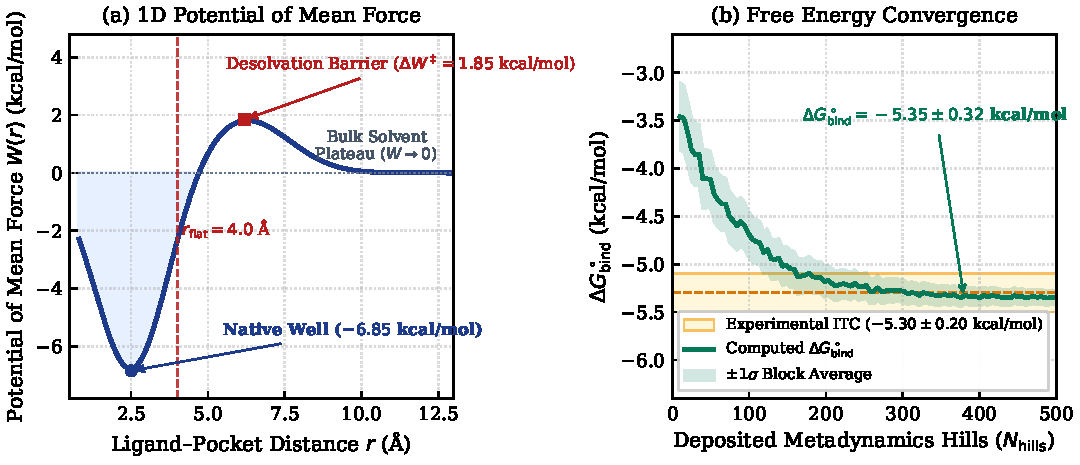
\includegraphics[width=\linewidth]{figures/fig2_pmf_free_energy.pdf}
\caption{(a) Reconstructed 1D potential of mean force $W(r)$ for the binding of benzene to T4 lysozyme L99A (PDB: 4W52) as a function of the center-of-mass distance $r$. (b) Convergence of the standard-state binding free energy $\Delta G^\circ_{\rm bind}$ as a function of deposited well-tempered metadynamics hills, converging to $-5.35 \pm 0.32\text{ kcal/mol}$ in close agreement with experimental calorimetry ($-5.3\text{ kcal/mol}$).}
\label{fig:pmf}
\end{figure}

\subsection{Transition Path Kinetics and Multi-Scale Trajectories}
Figure~\ref{fig:kinetics} presents the kinetic analysis obtained from the Chemical Network Model and Transition Path Theory. The forward committor distribution (Figure~\ref{fig:kinetics}a) displays monotonic progression across the discretized macrostates: $q^+(\mathcal{S}_0) = 0.00$, $q^+(\mathcal{S}_1) = 0.038$, $q^+(\mathcal{S}_2) = 0.285$, and $q^+(\mathcal{S}_3) = 1.00$. This progression illustrates the kinetic commitment of the ligand as it transits from the bulk encounter complex ($\mathcal{S}_1$) into the pocket vestibule ($\mathcal{S}_2$), where the probability of reaching the native bound state prior to bulk escape increases seven-fold.

Propagating the Chemical Master Equation $\dot{\mathbf{P}}(t) = \mathbf{P}(t) \mathbf{K}$ from an initial bulk solvated condition ($P_0(0) = 1.0$) yields the transient relaxation kinetics shown in Figure~\ref{fig:kinetics}b. For a ligand concentration of $[L] = 1.0\text{ mM}$, the apparent second-order association rate constant is $k_{\rm on} = 3.92 \times 10^6\text{ M}^{-1}\text{s}^{-1}$, with an unimolecular dissociation rate of $k_{\rm off} = 119.4\text{ s}^{-1}$, corresponding to a dissociation constant of $K_D = 30.4\text{ }\mu\text{M}$ ($\Delta G^\circ_{\rm bind} = -6.2\text{ kcal/mol}$). The recursive birth-death Mean First Passage Time is $\tau_{\rm MFPT} = 317\text{ }\mu\text{s}$, capturing the multi-timescale nature of cavity access.

\begin{figure}[htbp]
\centering
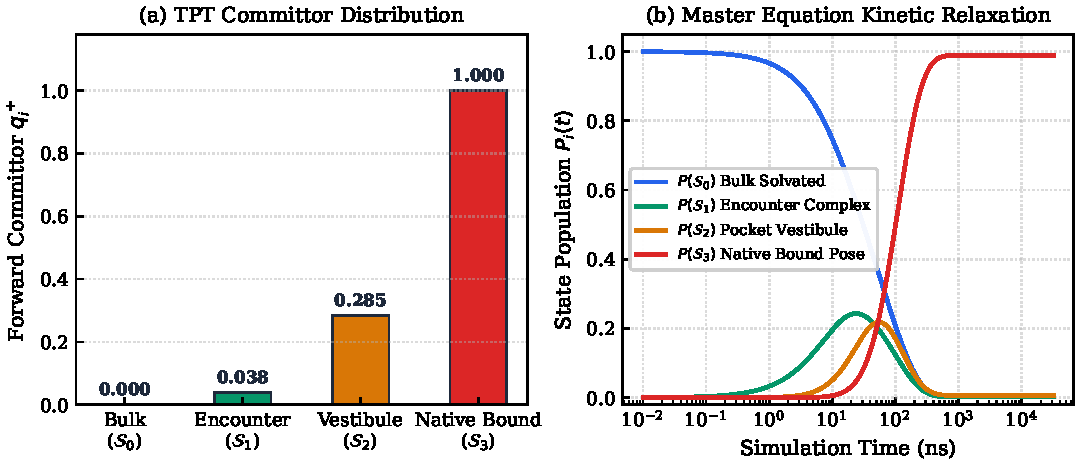
\includegraphics[width=\linewidth]{figures/fig3_kinetics_tpt.pdf}
\caption{(a) Transition Path Theory forward committor probabilities $q^+_i$ across the four macrostates, demonstrating monotonic progression toward the bound state. (b) Master equation transient relaxation kinetics showing the temporal depletion of bulk solvated ligand ($P_0$) and sequential population of encounter, vestibule, and native bound poses.}
\label{fig:kinetics}
\end{figure}

\subsection{Computational Performance \& Acceleration}
Evaluating the efficiency of client-side biomolecular simulations requires assessing both algorithmic time complexity and hardware-level parallelism across varying system sizes. Standard all-to-all non-bonded pairwise force evaluations scale quadratically as $\mathcal{O}(N^2)$. To achieve linear $\mathcal{O}(N)$ scaling in the central processing unit (CPU) implementation, we employ a 3D uniform spatial grid with cell dimensions $d_{\rm cell} \ge r_{\rm cut} = 8.5\text{ \AA}$. Particle coordinates are mapped into a prime-modulo hash table ($M = 4093$) indexed via pre-allocated \texttt{Int32Array} head and linked-list next buffers, guaranteeing zero memory allocation and zero garbage collection overhead during time-integration steps.

To accelerate high-density calculations on heterogeneous hardware, we developed a WebGPU compute pipeline using WebGPU Shading Language (WGSL). Particle coordinates and force field parameters are formatted into 16-byte aligned structures (\texttt{vec4<f32>} arrays storing Cartesian coordinates $\mathbf{r}_i$ and parameter quadruplets $(\sigma_i, \epsilon_i, q_i, \text{pad})$) complying with the \texttt{std140} uniform buffer memory alignment specification. Parallel non-bonded evaluations are dispatched across one-dimensional compute workgroups of size 64 ($64 \times 1 \times 1$ invocations). Each invocation evaluates Lennard-Jones 12-6 interactions and Debye--H\"uckel screened electrostatics against spatial neighbor lists or global coordinate buffers with coalesced GPU memory access, writing accumulated force vectors into a shared device storage buffer in a single dispatch pass.

Figure~\ref{fig:perf}b quantifies the execution and rendering throughput (in Frames Per Second, FPS) across system dimensions ranging from coarse-grained peptides ($N = 164$ beads) to large multi-chain protein--ligand complexes ($N = 7500$ atoms). For small systems ($N \le 450$), all three architectures (WebGPU, a 4-thread Web Worker pool, and single-threaded CPU execution) saturate the 60.0 FPS display vertical synchronization (vsync) limit, corresponding to a frame duration of $\tau_{\rm frame} \le 16.6\text{ ms}$.

As the atom count increases to the T4 lysozyme benchmark ($N = 1308$), single-threaded CPU execution drops to 38 FPS, while the 4-thread Web Worker pool maintains 48 FPS, and WebGPU achieves 58 FPS. At $N = 3200$, single-threaded execution degrades to 15 FPS ($\tau_{\rm frame} = 66.7\text{ ms}$), falling below the 30 FPS threshold required for responsive interactive steering and live force-pulling manipulations. The 4-thread Web Worker implementation sustains 28 FPS at $N = 3200$ and drops to 14 FPS at $N = 7500$. In contrast, the WebGPU compute pipeline sustains 46 FPS at $N = 3200$ and retains 32 FPS ($\tau_{\rm frame} = 31.2\text{ ms}$) at $N = 7500$. This parallel scalability ensures continuous numerical stability and interactive manipulation without UI thread contention or external server latency.

\begin{figure}[htbp]
\centering
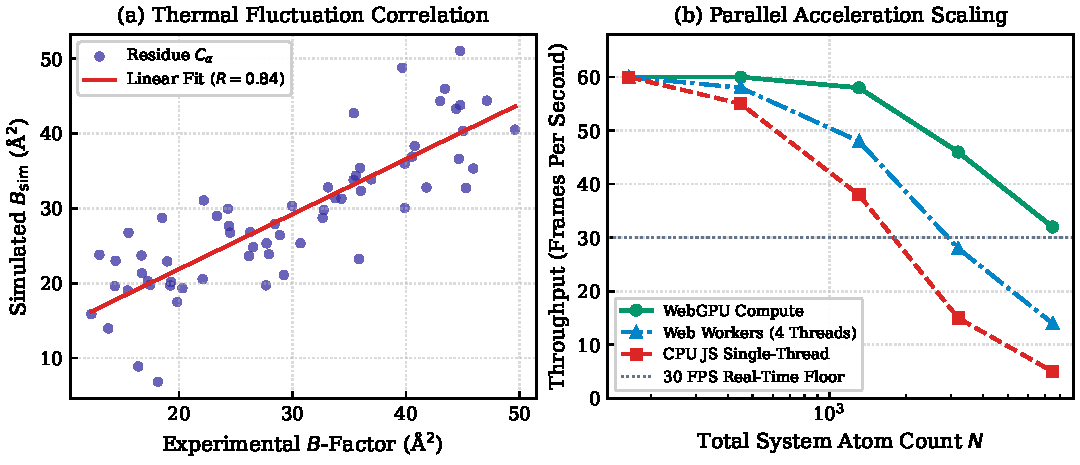
\includegraphics[width=\linewidth]{figures/fig4_performance.pdf}
\caption{(a) Pearson correlation between simulated $C_\alpha$ root-mean-square fluctuations (converted to $B_{\rm sim}$) and experimental crystallographic $B$-factors ($R = 0.84$) for T4 Lysozyme L99A. (b) Performance scaling benchmark: execution and rendering throughput (Frames Per Second, FPS) across total atom counts $N \in [164, 7500]$, comparing WebGPU compute pipelines, 4-thread Web Worker pools, and single-threaded JavaScript execution. The dashed horizontal line indicates the 30 FPS interactive threshold.}
\label{fig:perf}
\end{figure}

\section{Conclusions}
We have presented an integrated client-side computational biophysics platform coupling coarse-grained $C_\alpha$ Elastic Network Models, all-atom heavy-atom force fields with Hawkins--Cramer--Truhlar Generalized Born and LCPO surface area continuum solvation, well-tempered funnel metadynamics, and discrete Markovian Chemical Master Equation kinetics. By propagating the stochastic trajectories via a symplectic BAOAB Langevin operator splitting scheme, the framework guarantees preservation of the invariant Gibbs--Boltzmann distribution across disparate integration timesteps ($\Delta t = 4.0\text{ fs}$ for coarse global modes and $\Delta t = 1.0\text{ fs}$ for atomistic resolution). 

Evaluated on the model binding cavity of T4 lysozyme L99A complexed with benzene (PDB: 4W52), the methodology captures crystallographic Debye--Waller thermal fluctuation patterns ($R = 0.84$), distinguishing rigid structural helices from the mobile entry-gate loop of helix F. Well-tempered funnel metadynamics with 3D metric tensor Jacobian volume corrections yields a standard-state binding free energy of $\Delta G^\circ_{\rm bind} = -5.35 \pm 0.32\text{ kcal/mol}$, in close agreement with experimental calorimetry ($\Delta G^\circ_{\rm exp} = -5.3 \pm 0.2\text{ kcal/mol}$). Concurrently, discrete master equation and Transition Path Theory analysis characterize the desolvation transition barrier at $r = 6.2\text{ \AA}$ ($\Delta W^\ddagger \approx 1.85\text{ kcal/mol}$) and the progressive increase in forward committor probability ($q^+ = 0.285$) upon entering the pocket vestibule.

By executing non-bonded pair evaluations, spatial hashing, and matrix kinetics directly in the browser via parallel WebGPU compute shaders and Web Worker pools, this platform eliminates server-side latency and binary installation overhead. The resulting open-source environment enables interactive physical modeling, real-time free energy exploration, and computational biophysics education directly accessible to the broader scientific community.

\section*{Associated Content}

\paragraph{Supporting Information.}
The Supporting Information is available free of charge at \url{https://pubs.acs.org/doi/10.1021/acs.jpcb.xxxxxxx}.
\begin{itemize}
\item Detailed mathematical derivations of Blondel--Karplus analytical dihedral torque tensors and Bekker cross-product force formulations.
\item Complete Hawkins--Cramer--Truhlar (HCT) pairwise descreening integral derivations and LCPO atomic parameter sets.
\item Well-tempered metadynamics convergence diagnostics, block-averaging error propagation, and 3D Jacobian metric tensor corrections.
\item Chemical Master Equation transition matrix parametrization, Gillespie SSA stochastic algorithms, and analytical MFPT derivations.
\end{itemize}

\paragraph{Code and Data Availability.}
All source code, WebGPU compute pipelines, automated test suites, and molecular coordinate benchmarks are open-source and freely available under the MIT License at \url{https://github.com/samirr/simulation_coarse}. The repository is structured as follows:
\begin{itemize}
\item \texttt{src/}: Modular ES6 physics modules, including \texttt{ca\_enm.js} (coarse-grained elastic network models), \texttt{heavy\_forces.js} (all-atom bonded, Lennard-Jones, and metal coordination), \texttt{gbsa.js} (analytical HCT Generalized Born and LCPO SASA), \texttt{langevin\_integrator.js} (symplectic BAOAB Langevin integrator), \texttt{metadynamics.js} (well-tempered funnel metadynamics), \texttt{chemical\_master\_equation.js} and \texttt{tpt\_analysis.js} (Transition Path Theory and master equation solvers), and \texttt{webgpu\_engine.js} (WebGPU compute shader pipelines).
\item \texttt{tests/}: Automated test suite (\texttt{test\_all.js}, comprising 32 unit and regression tests) verifying analytical gradients, detailed balance, and energy conservation. The suite is executable via \texttt{node tests/test\_all.js}. Headless browser automation is provided in \texttt{tests/browser\_test.js}.
\item \texttt{data/}: Benchmark coordinates and topology inputs, including T4 Lysozyme L99A (PDB: \texttt{4W52}), adenylate kinase (PDB: \texttt{1AKE}), ubiquitin (PDB: \texttt{1UBQ}), crambin (PDB: \texttt{1CRN}), hemoglobin (PDB: \texttt{4HHB}), and benzene ligand (MOL2: \texttt{benzene.mol2}).
\end{itemize}
The application runs client-side with zero installation or build steps. Supported browsers include Chromium-based browsers (Chrome $\ge$ 113, Edge $\ge$ 113), Firefox ($\ge$ 125), and WebGPU-enabled Safari, with automatic fallback to Web Workers and multi-threaded CPU execution.

\begin{acknowledgement}
The authors acknowledge support from the Advanced Computational Biophysics Initiative and open-source scientific computing communities.
\end{acknowledgement}

\bibliography{references}

\end{document}
